\chapter{Literature Survey}

The outline of the chapter should be as follows:


English is the most heavily studied language by the NLP community and hence most of the tools for syntactic analysis have been developed keeping English and its treebanks in consideration. The techniques which have been developed for English do not naturally extend to many other languages like German, Hindi, Hebrew, Arabic, etc \cite{tsarfaty2010statistical}. These languages belong to a different class and are known as morphologically rich languages (MRLs). In this research question, I want to explore techniques that can be used for constituency parsing of MRLs. We will begin by understanding what are MRLs and what properties distinguish them from English in section \ref{sec:mrl}. In section \ref{sec:joint}, we will look at why joint morphological and syntactic analysis is important for MRLs and in section \ref{sec:lattice}, we will look at how it is done using lattices of part-of-speech tags.

\section{Morphologicall Rich Languages}
\subsection{What are MRLs?}
\label{sec:mrl}

A morpheme is the minimal meaning-bearing unit in a language. Multiple morphemes can be combined together to form new words in many different ways such as inflection, derivation, and cliticization. In NLP, morphology is the study of the way the words are built by the combination of one or more morphemes \cite{Jurafsky:2009:SLP:1214993}. A given word could thus contain multiple syntactic constituents with different syntactic functions. In relation to this, syntactic parsing operates at a higher level and uncovers the role of individual syntactic constituents and also the relations between various constituents. In a configurational language such as English, such syntactic information is conveyed through the order of constituents or words in the sentence. On the contrary, morphologically rich languages are those languages which convey such information by word formation (via inflection, cliticization, etc.) instead of word order \cite{seddah2013overview}. For instance, subject-predicate dependency is revealed by agreement on number and gender expressed by word morphology instead of their relative positions in the sentence. Owing to the above fundamental difference, MRLs tend to have a relatively \textit{free word order} i.e. the words in a sentence are free to change their positions without changing the meaning of the sentence. The non-rigid structure of parse trees owing to the free word order and morphological ambiguity due to a rich morphology are the major challenges of parsing MRLs. As has been pointed earlier, boundaries of constituents of the syntactic structure need not coincide with word boundaries as it happens in English.

\subsection{Joint inference of morphology and syntax}
\label{sec:joint}
In a typical NLP pipeline for English, first, the morphological analysis of the words of the sentence is performed which is followed by labelling the constituents with part-of-speech tags and eventually followed by syntactic parsing. But MRLs, owing to their nature, render such a pipeline ineffective. As was mentioned in the previous section, the boundaries of constituents need not coincide with word boundaries, as words can be made up multiple morphemes. Moreover, due to the existence of discontinuous constituents in MRLs, each of the constituents can play a variety of different syntactic roles. It has been pointed out by \cite{tsarfaty:2006} that there is a lot of ambiguity in each of the steps in the pipeline for MRLs. To disambiguate syntactic analysis (parsing), information needs to flow from the morphological analysis (segmentation) towards it, whereas, for disambiguation of morphological analysis, information needs to flow from syntactic analysis towards it. The common ground which connects these two tasks is part-of-speech tagging. Thus for an effective system, information should flow in both directions: $segmentation \rightarrow tagging \rightarrow parsing$ as well as $parsing \rightarrow tagging \rightarrow segmentation$.

This can be achieved by performing a joint morphological and syntactic analysis. Consider a sentence of $m$ words represented as  $w_1^m$. Let this sentence be segmented in $n$ constituents represented by $s_1^n$. Let the sequence of tags associated with every segment be denoted by $t_1^n$. Finally, let the parse tree be denoted by $\pi$. The goal of the joint morpho-syntactic analysis is shown in equation \ref{eq:joint_1}. This can be broken down into various components as shown in equation \ref{eq:joint_2}

\begin{align}
    \label{eq:joint_1}
    {\langle \pi, t_1^n, s_1^n \rangle}^* &= \argmax_{\langle \pi, t_1^n, s_1^n \rangle} p({\langle \pi, t_1^n, s_1^n \rangle} | w_1^m) \\
    &= \argmax_{\langle \pi, t_1^n, s_1^n \rangle} \underbrace{p(\pi \mid t_1^n, s_1^n, w_1^m)}_\text{parsing} \underbrace{p(t_1^n \mid s_1^n, w_1^m)}_\text{tagging} \underbrace{p(s_1^n \mid w_1^m)}_\text{segmentation}
    \label{eq:joint_2}
\end{align}

\cite{cohen:smith:2007} proposed a system that performs joint inference using factored models for morphology and syntax, which are designed and trained individually.


\subsection{Lattice parsing}
\label{sec:lattice}

Consider a word $w$ which has two possible segmentations i.e. it can either be segmented as $(s_1, s_2)$ with corresponding POS tags $(t_1, t_2)$ or the entire word can act as a single segment $s_3$ with $t_3$ as the corresponding POS tag. Information which tells us which what the right segmentation is, lies in the syntactic analysis of the sentence. But, at the same time, we need the right segmentation in order to perform the right syntactic analysis. In a traditional sequential analysis, either the segmentation having greater likelihood (as calculated from the treebank) will be preferred or the model will just take into account their likelihoods without the syntactic context. To avoid this, \cite{goldberg:tsarfaty:2008} introduced the idea of lattice parsing, in which, instead of parsing over a fixed input sentence, the parser operates on a structure of all possible segmentations called the lattice.

The idea of representing ambiguity as lattice structures is inspired by the speech recognition community \cite{chappelier:etal:1999} where it represents the different possible sentences resulting from an utterance based on the acoustic model. In our situation, it represents all possible segmentation and corresponding POS tags for a given sentence. A path through the lattice represents one possible morphological segmentation of the given sentence. Consider an example lattice representation of the Hebrew phrase \textit{bclm hneim} as presented by \cite{goldberg:tsarfaty:2008} as shown in figure \ref{fig:lattice}.

\begin{figure}[htb]
    \centering
    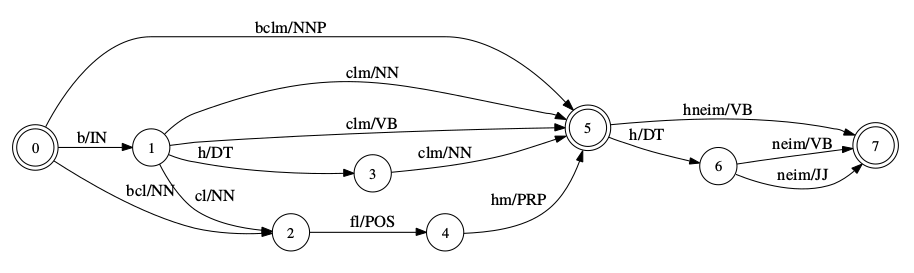
\includegraphics[scale=0.47]{lattice}
    \caption{The Lattice for the Hebrew phrase \textit{bclm hneim}}
    \label{fig:lattice}    
\end{figure}

The traditional PCYK algorithm for constituency parsing was extended to accept lattice inputs and to search over all lattice paths instead of just words in a sentence. \cite{goldberg:elhadad:2011} and \cite{green:manning:2010} have shown that doing so increases the parsing accuracy for Hebrew and Arabic respectively. In shift-reduce constituency parsing, most work either assume that they have access to gold segmentation and tagging labels or perform segmentation and tagging as a precursor to parsing, which hurts the parsing accuracies. The standard shift-reduce parsing algorithm for constituency parsing can also be modified to incorporate tag-lattices as inputs instead of plain sentences. It has been done for Chinese by \cite{wang2014joint} whereas \cite{mi2015shift} used for English and Chinese.